% Design and System Architecture
\section{Design}
\label{sec:design-and-system-architecture}

This chapter will discuss the design and system architecture of the project. The project is divided into three main components: the mechanical design, the integration of electronics and software, and the computer vision system. The mechanical design will be discussed in \autoref{sec:mechanical-design}, the electronics and software integration in \autoref{sec:electronics-and-software-integration}, and the computer vision system in \autoref{sec:computer-vision-system}.

\subsection{System Architecture}
\label{sec:system-architecture}

The project's design is underpinned by a modular design philosophy; each subsystem is designed to be as independent as possible, allowing for easier debugging and maintenance, and expose only high level interfaces to other subsystems. This not only simplifies the development process but also allows for easier integration of new features in the future.

\begin{figure}[H]
    \begin{minipage}[h]{\textwidth}
        \centering
        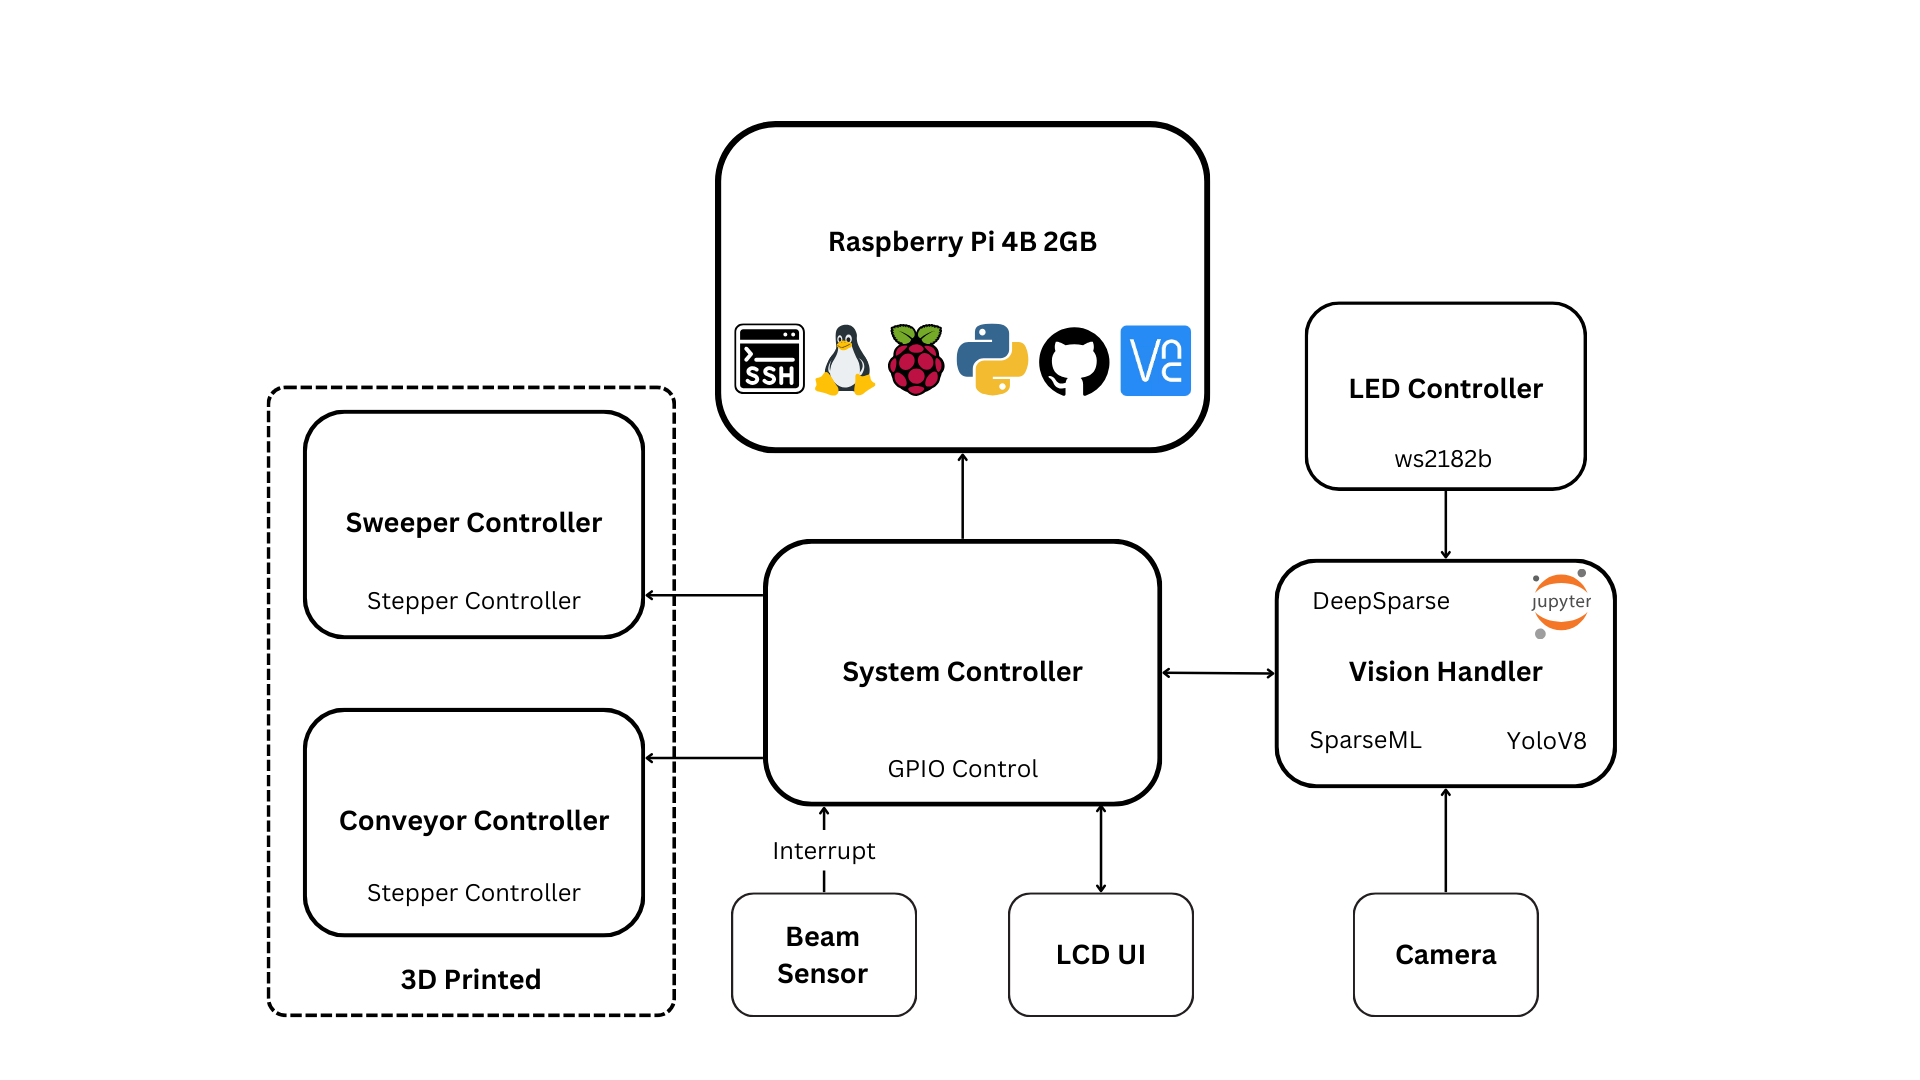
\includegraphics[height=10cm]{imgs/diagrams/System Diagram.png}
        \caption{System Architecture Diagram}
    \end{minipage}
\end{figure}

A System Controller oversees the entire system, interacting with all other components and controlling all communication. It is responsible for interacting with the Vision Handler, and passing commands to the Conveyor Controller and Sweeper Controller. The Vision Handler is responsible for processing images from the camera and performing inference for classification. The Conveyor Controller is responsible for controlling the conveyor belt, while the Sweeper Controller is responsible for controlling the sweeper. Both of these controllers also control a TMC2209 stepper motor driver, which in turn controls the stepper motors that drive the conveyor belt and the sweeper.

There is two-way communication between the LCD UI and System Controller as the user may input commands to the system, and the System Controller may send status updates to the LCD UI.

\subsection{Hardware}
\label{sec:hardware}

When selecting hardware for the project, it is vital to consider the requirements of the system and to evaluate the trade-offs between alternatives. This section will detail the choice of hardware and provide justification for the selection.

\subsubsection{Raspberry Pi 4 Model B}
The Raspberry Pi 4 Model B \cite{pi4} was chosen as the main component of the system and is the central hub that all other components are connected to. This model was chosen as it is regarded as a reliable SoC (System on Chip) and is widely used in the industry. It has a large amount of software and driver support, ensuring confidence in finding solutions to problems encountered over the course of the project. Additionally, it has GPIO pins that can be used to control the other components in the system, such as stepper motors and LEDs. It also has a dedicated CSI port which allows for a camera to be connected directly to the SoC, which is necessary for the computer vision system.

\begin{figure}[H]
    \begin{minipage}[t]{\textwidth}
      \centering
      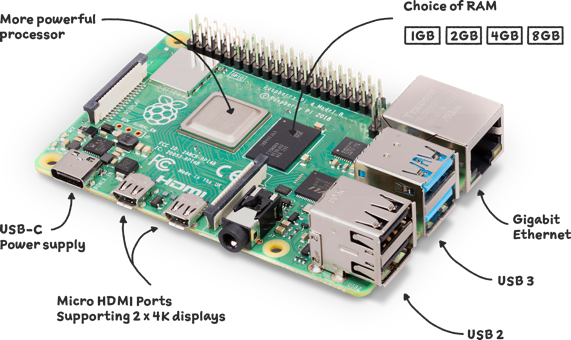
\includegraphics[width=\textwidth,height=5cm, keepaspectratio]{imgs/parts/pi4_labelled.png}
      \caption{Raspberry Pi 4 Model B 2GB \cite{pi4}}
    \end{minipage}
\end{figure}

It also features Wi-Fi support, allowing for SSH and remote development software, as well as an HDMI port for the display. Originally, the 4 GB model was to be used however an order issue resulted in receiving the 2 GB model. This was found to be not an issue as the 2 GB model still performed well, but there was now a heavier need for efficient code to ensure the system runs smoothly.

An alternative to the Pi family of SoCs could be an Arduino-compatible microcontroller, but while they are capable of controlling the components of the system, and potentially drive an LCD, they lack the resources to run the Computer Vision system and stream video from the camera. Due to this, they cannot be used as a replacement for the Pi. It was considered to use an Arduino-compatible microcontroller to delegate control of certain components to overload the Pi, but this was found to be unnecessary as the Pi was able to handle the load of the system.

A viable alternative to the Pi could be a Nvidia Jetson Nano \cite{jetsonnano}, as it is designed for Computer Vision applications and has a dedicated GPU. The dedicated GPU would reduce the likelihood of the Computer Vision system being a bottleneck, and it has a CSI port for the camera. In terms of CPU performance, the Nano is weaker than the Pi, having a quad-core ARM Cortex-A57, whereas the Pi has a quad-core ARM Cortex-A72\cite{pi4}. However, the worse CPU performance is offset by the dedicated GPU, and the Nano has 4 GB of RAM, making the Nano a very attractive alternative to the Pi. The Nano's drawback is that it is significantly more expensive than the Pi (up to 3x from retailers), and
given the ability to optimise the computer vision system as discussed in \autoref{sec:background} (Background), the Pi is still a viable choice for the computer vision system.

To address the lack of a dedicated GPU for inference on the Pi, an article from Medium\cite{benchmarks} benchmarked the Pi's performance on various computer vision tasks with various accelerators like the Intel Neural Compute Stick 2 and the Google Coral USB Accelerator against other SoCs like the Jetson Nano and the Coral Dev Board. It was found that the Coral Dev Board was the best performing, however the Pi using optimisation libraries like TensorFlow Lite showed promising results, which helps to strengthen the argument for using the Pi for the computer vision system, especially with the SparseML and DeepSparse libraries that were discussed in \autoref{sec:background} (Background).

The benchmarks can be found in Appendix \autoref{app:benchmarking}.

\subsubsection{DFRobot 7" Touchscreen Display}
The DFRobot 7" Touchscreen Display was chosen for the LCD panel as it is a relatively cost-effective display that is compatible with the Raspberry Pi. It has touchscreen support and features Raspberry Pi 4 mounting holes on its back, as well as HDMI adapter boards to connect to the Pi. This means that a physical mount for the Pi does not need to be designed, and only a mount for the display is required. The display is also powered by the Pi, so no additional power supply is required. 

\begin{figure}[H]
    \begin{minipage}[t]{\textwidth}
      \centering
      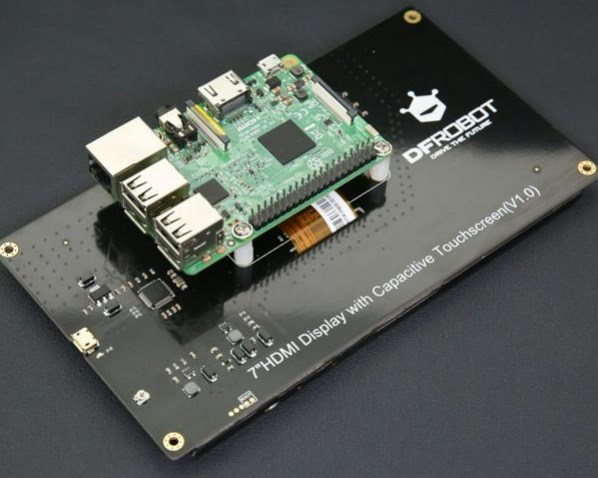
\includegraphics[width=\textwidth,height=5cm, keepaspectratio]{imgs/parts/dfrobot_screen.jpg}
      \caption{DFRobot 7" Touchscreen Display \cite{7inchdisplay}}
    \end{minipage}
\end{figure}

Other alternatives to the DFRobot 7" display were various 10" displays however many required proprietary drivers and cables, and were more expensive. The inclusion of mounting holes on the back of the DFRobot display was also a major factor in its selection, which seems to be uncommon in other displays.

\subsubsection{Okdo Adjustable Focus OV5647 Camera}
For the Computer Vision system, a camera is required to capture images of the components. The Okdo Adjustable Focus OV5647 Camera was chosen as it is CSI compatible, meaning it can be connected directly to the Raspberry Pi, and has a manual focus ring, allowing it to be used as a macro camera to capture images of small components placed directly above it. The manual focus ring allows the focus of the camera to be specifically tuned to the design of the system, allowing for the best possible image quality. It also has a 5MP sensor\cite{okdospec}, which is sufficient for the Computer Vision system, as high-resolution images would be preprocessed and reduced, only adding to the amount of processing required.

\begin{figure}[H]
    \begin{minipage}[t]{\textwidth}
      \centering
      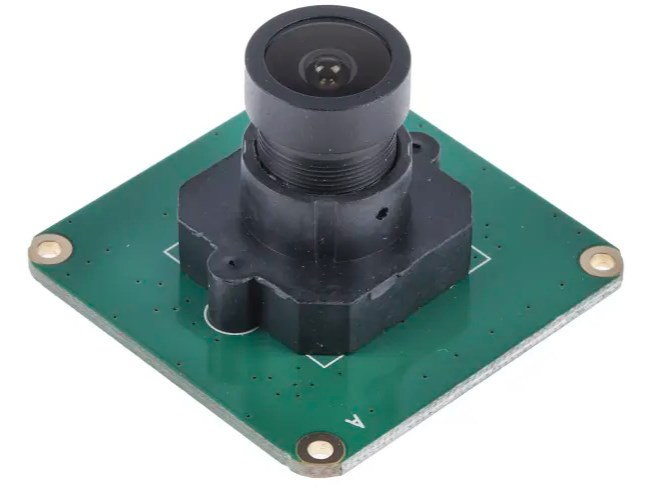
\includegraphics[width=\textwidth,height=5cm, keepaspectratio]{imgs/parts/okdo_camera.jpg}
      \caption{Okdo Adjustable Focus OV5647 Camera \cite{okdocamera}}
    \end{minipage}
\end{figure}

Other cameras were considered, such as the Raspberry Pi Camera Module V2 \cite{picamerav2}, however, it lacks a manual focus ring, which may result in a Minimum Object Distance (the closest distance at which an object can be captured) that is too far for the design of the system. Another camera, the Raspberry Pi High Quality Camera \cite{picamerahq} also has the option of replacing the lens with a dedicated macro lens, however these are incredibly expensive.

\subsubsection{WS2812B LEDs}
To illuminate the components on the conveyor belt, a solution was required that could provide bright, controllable light. The WS2812B LEDs \cite{ws2812b} were chosen as they are individually addressable, meaning that each LED can be controlled independently, allowing for a wide range of colours and patterns to be displayed. They are also relatively cheap and easy to source, and are compatible with the Raspberry Pi and have a large amount of support due to their popularity. They also can run off 5V, meaning it can share the input power rail with the Raspberry Pi and are also easy to control, requiring only a single GPIO pin to control many LEDs as they can work with either SPI or PWM signals, depending on the chosen library.

\begin{figure}[H]
    \hfill
    \begin{minipage}[t]{0.45\textwidth}
      \centering
      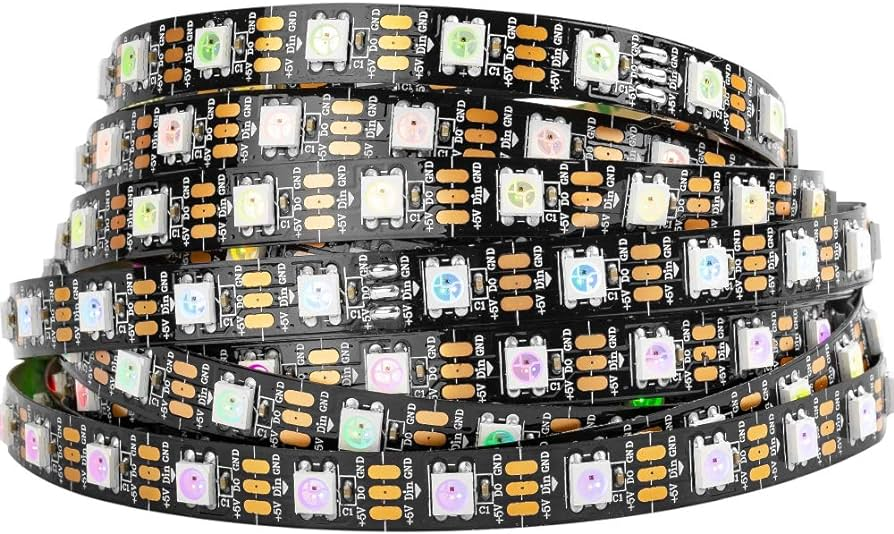
\includegraphics[width=\textwidth,height=5cm, keepaspectratio]{imgs/parts/ws2812b.jpg}
        \caption{WS2812B LEDs \cite{ws2812b}}
    \end{minipage}
    \hfill
    \begin{minipage}[t]{0.45\textwidth}
        \centering
        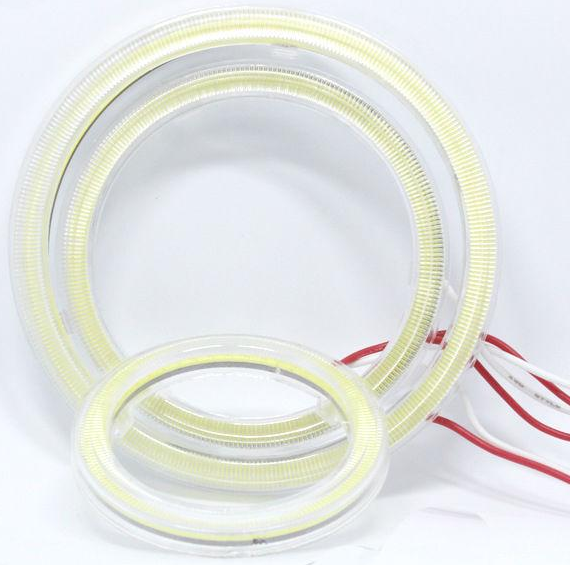
\includegraphics[width=\textwidth,height=5cm, keepaspectratio]{imgs/parts/cob.jpeg}
        \caption{12V COB Ring Light}
      \end{minipage}
      \hfill
\end{figure}

Originally, a 12V COB ring light was considered, as it could produce a uniform light source, however the specific ring was not dimmable and resulted in strange flickering when attempting to do so with a MOSFET. It also did not produce a clean white light, but a more blue light. The WS2812B LEDs were chosen as they could produce any light colour, and could be cut and placed in any configuration, allowing for a more customisable design.

\subsubsection{Stepper Motors}
Stepper motors possess the ability to move in precise increments, making them ideal for the Sweeper System which requires precise control. The Conveyor System is not as demanding, but stepper motors were chosen for consistency across the system. The NEMA17 series of stepper motors were chosen \cite{nema17} as they are widely used and have a large amount of support and documentation, also typically used in FDM printers. With the ability to rotate at 1200RPM/900RPM at 12V, and a holding torque 48/63Ncm (for single/double stack motors), they are more than capable of driving the conveyor belt and sweeper arm.

\begin{figure}[H]
    \hfill
    \begin{minipage}[t]{0.45\textwidth}
      \centering
      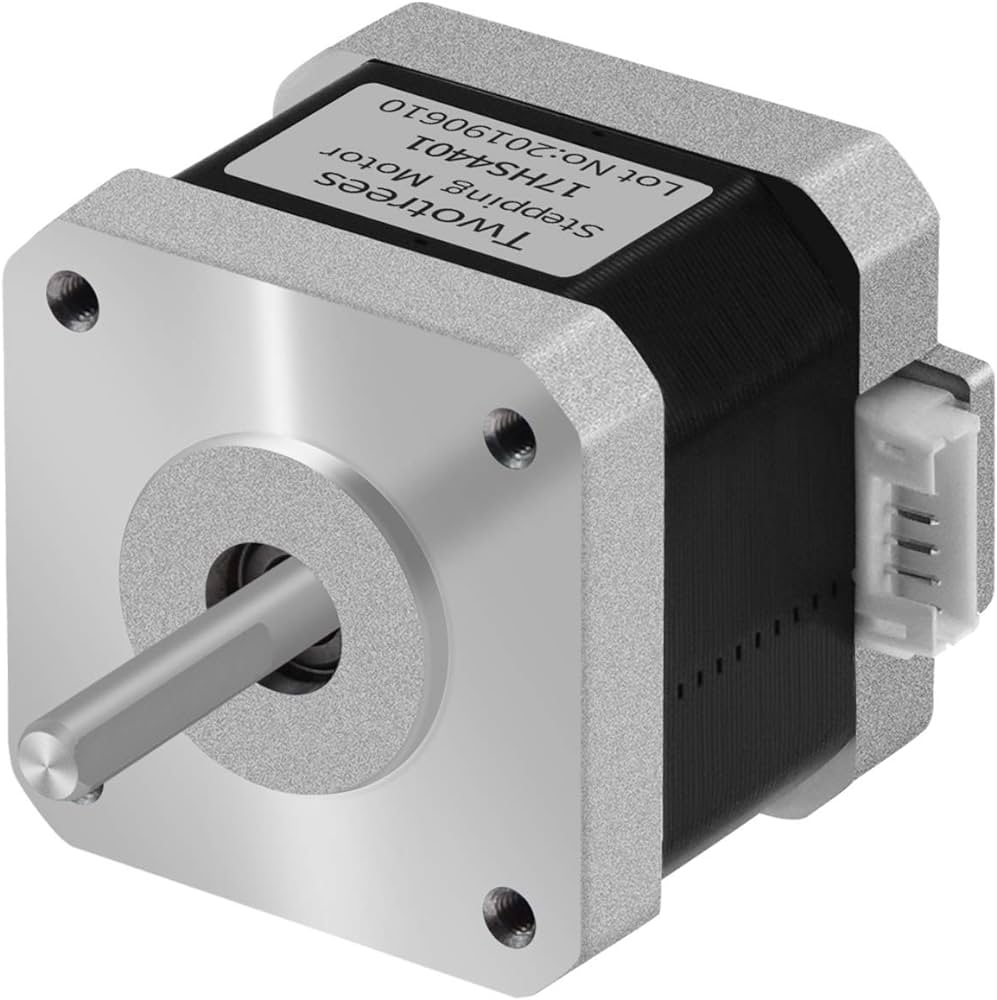
\includegraphics[width=\textwidth,height=5cm, keepaspectratio]{imgs/parts/nema17.jpg}
      \caption{NEMA17 Stepper Motor \cite{nema17}}
    \end{minipage}
    \hfill
    \begin{minipage}[t]{0.45\textwidth}
        \centering
        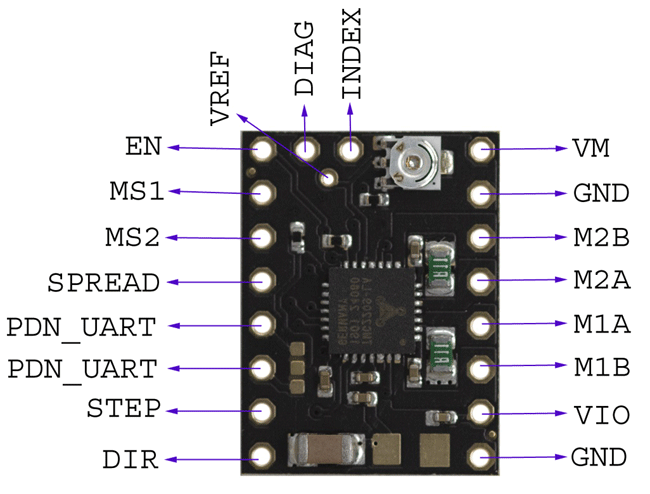
\includegraphics[width=\textwidth,height=5cm, keepaspectratio]{imgs/parts/tmc2209.png}
        \caption{TMC2209 Stepper Motor Driver \cite{tmc2209}}
      \end{minipage}
      \hfill
\end{figure}

For driving the motors, TMC2209s were selected due to their microstepping support and silent operation. Due to their popularity in FDM printing and the ease of use, they have a large amount of support and documentation. They are also capable of driving the NEMA17 series of stepper motors, and are compatible with the Raspberry Pi. Originally, the DRV8825 was considered \cite{drv8825}, however they added significant noise to the system and were unpleasant to use.

\subsubsection{Break Beam Sensor}

Due to the complexity of the system, it is vital to ensure that the system is as efficient as possible to ensure real-time performance. The design choice was made to use an IR Beam Break Sensor \cite{breakbeamsensor} to detect the presence of objects on the conveyor belt to reduce the computational overhead of constant inference on the Vision Handler. The System Controller connects directly to the IR Beam Break Sensor, which is used to detect the presence of objects on the conveyor belt, making use of interrupts to detect changes in the sensor's state. This allows for a fast response from the system without much computational overhead. The sensor itself does not change lighting conditions as it operates with infrared light, which is not visible to the human eye. The sensor is also easy to install and maintain, as it only requires a power supply and a digital input pin to operate.

\begin{figure}[H]
    \begin{minipage}[h]{0.95\textwidth}
        \centering
        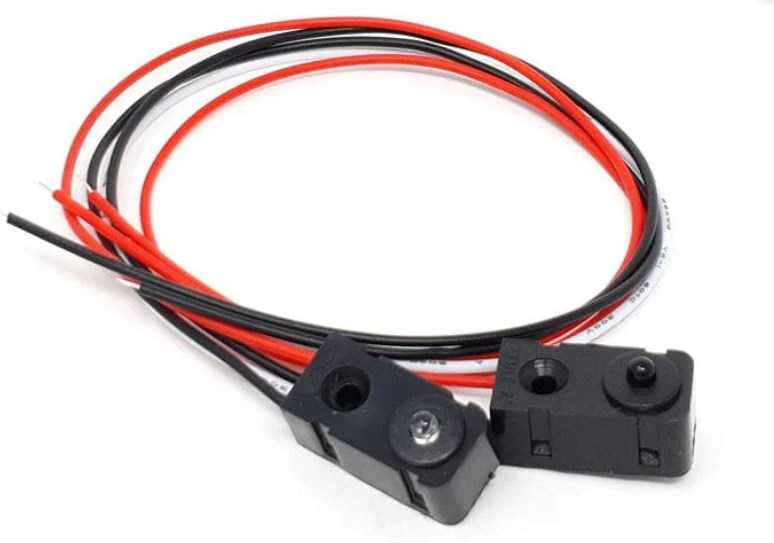
\includegraphics[height=6cm]{imgs/parts/breakbeam.jpg}
        \caption{IR Beam Break Sensor}
    \end{minipage}
\end{figure}

An alternative to the IR Beam Break Sensor would be to use software approaches on the Vision Handler to detect the presence of objects on the conveyor belt, for example using OpenCV to detect large changes between successive frames. This could be implemented in a number of ways such as background subtraction or histogram comparison. However, this would also require the Vision Handler to constantly process frames, which would increase the computational overhead of the system. The IR Beam Break Sensor is a more efficient solution as it allows the system to only process images when an object is detected on the conveyor belt.

An approach to dynamically adjust the frame rate of the camera could be considered, increasing frame rates when there are no objects on the conveyor belt in anticipation of objects being placed on the conveyor belt, and reducing frame rates when objects are detected to reduce computational overhead. This could potentially impose resource contention between the Vision Handler and the System Controller while it is controlling the Sweeper and Conveyor Belt. The framerate also needs to take into consideration the conveyor speed to not miss objects, requiring both more complexity and computational resources.

An alternative to the IR Beam Break Sensor would be to use a proximity sensor to detect the presence of objects on the conveyor belt, however this requires constant polling which would be less efficient than using an interrupt-based approach. Additionally, the IR Beam Break Sensor is a more reliable solution as it is less prone to false positives than a software-based approach. The IR Beam Break Sensor is a more robust solution as it is less prone to interference from external factors such as lighting conditions or shadows.

For these reasons, the IR Beam Break Sensor was chosen as the best solution for detecting the presence of objects on the conveyor belt.

\subsubsection{Power Supply Unit}
To power the system, two parameters were taken into account when choosing a PSU; the power rating and voltage.

\begin{figure}[H]
    \begin{minipage}[h]{0.95\textwidth}
        \centering
        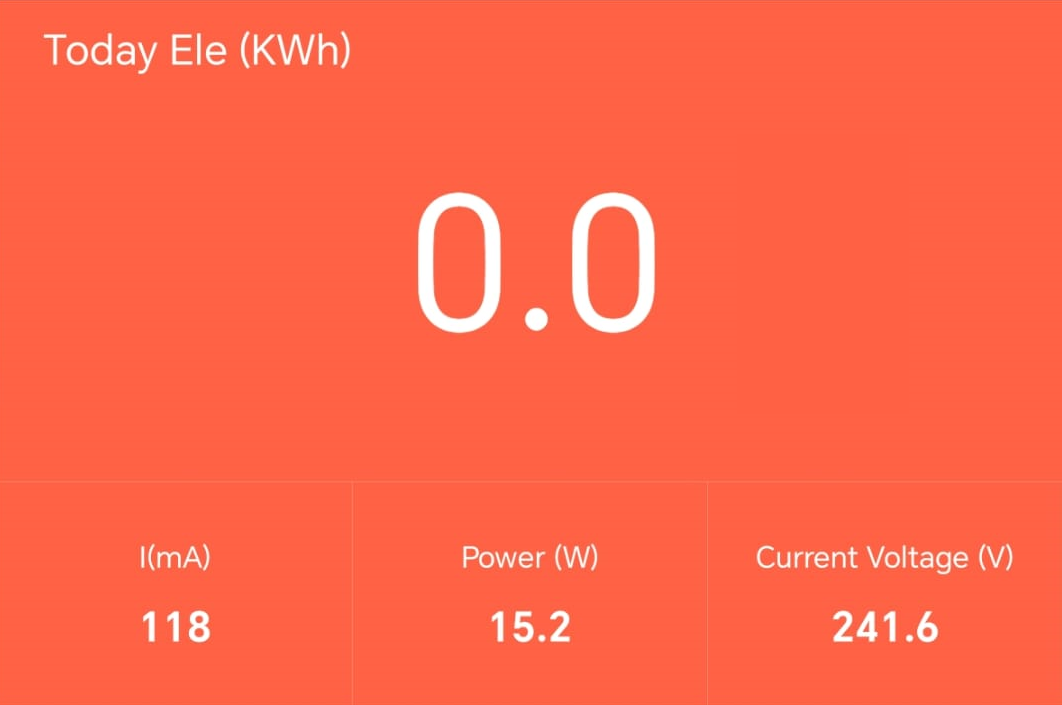
\includegraphics[height=5cm]{imgs/parts/powermeter.png}
        \caption{Power consumption of the system}
        \label{fig:powermeter}
    \end{minipage}
\end{figure}

Firstly, the power supply must be able to drive all components in the system with overhead in case of spikes in power consumption. The system consists of a Raspberry Pi 4 Model B, a DFRobot 7" Touchscreen Display, two NEMA17 stepper motors and TMC2209 stepper motor drivers, an IR Beam Break Sensor, an Okdo Adjustable Focus OV5647 Camera, and 16 WS2812B LEDs. 

In the early stages of the project, with only the Raspberry Pi, the DFRobot 7" Touchscreen Display, WS2812B and Okdo Camera, the power consumption was measured to be under 20W, recorded using a smart plug with a power meter as shown in \autoref{fig:powermeter}. It was thought that the addition of the NEMA17 motors and TMC2209 stepper motors would contribute ~50W (running at 2A 12V) to the power consumption, making for a power consumption of under 70W. A 30W overhead would have been added to the power supply, resulting in a 100W power supply. However, a 150W power supply was used instead due to an overestimation on the power consumption of the system before finalising the design. In hindsight, the 150W power supply was excessive, and a 100W power supply would have been sufficient.

\todo{add power consumption measurements from usb for complete power - implementation maybe?}

Additionally, the voltage of the power supply must be greater than or equal to the highest voltage of any component in the system to enable the use of step down convertors to power the components. The highest voltage of any component in the system is 12V and the lowest is 5V. Initially, 24V components were a possibility due to the variety of LEDs and stepper motors, so a 24V power supply was chosen.

This resulted in selecting a 24V DC 6.25A Power Supply Unit.

\subsubsection{Step Down Convertors}

\subsection{Software}
\label{sec:electronics-and-software-integration}

\subsubsection{Conveyor Controller}
\label{sec:conveyor}

\subsubsection{Sweeper Controller}
\label{sec:sweeper}

\subsection{Mechanical Design and Electronics}
\label{sec:mechanical-design}
As the system has a major physical component, the mechanical design is a crucial aspect of the project. The mechanical design is responsible for the physical structure of the system, including the conveyor system, the sweeper, bins, the housing for the LCD and PSU (Power Supply Unit), and the camera mount. It provides the foundation for the system to operate and interact with the environment, and as such it is important to ensure that the mechanical design is robust and reliable.

The system also has a major electronics component due to the requirement of moving parts, namely the conveyor and sweeper systems. Care must be taken to ensure that the power delivery to these systems is stable and reliable, and connections are secure. Careful consideration must also be taken to ensure electrical safety, preventing damage to the system and harm to the user. 

The system has been designed in FreeCAD \cite{freecad}, a free and open-source parametric 3D CAD software. Aligning with the modular design approach of the project, the parametric nature of FreeCAD allows for easy modification of the design by modifying numerical parameters, which is useful in designs that require frequent changes. It was decided to use FDM printing to produce the components of the system using PLA, a biodegradable thermoplastic derived from renewable resources such as corn starch or sugarcane. PLA is easy to print, and does not require ventilation or post-processing, unlike other materials like ABS\cite{fdmmaterials}. The known brittleness and low heat resistance of PLA are not a concern for this project, as the system is not exposed to high temperatures or direct mechanical stress. An alternative to PLA would be PETG, which has higher heat resistance and is less brittle than PLA, however, it is more difficult to print and is more prone to warping - it is also less environmentally friendly than PLA and less cost effective.

All components are designed to be easily assembled and disassembled, allowing for easy maintenance and repair. They are easily assembled using standard M3 screws and brass inserts, which are easy to source and replace. 


\subsubsection{Conveyor}
\label{sec:conveyor-design}
As discussed in the Background (\autoref{sec:background}), a conveyor belt system with a face down camera seems to be the most promising approach. For the design of the conveyor system, it is imperative that the following requirements are met:
\begin{mylist}
    \item The conveyor belt must be able to move objects from the input to the output.
    \item The conveyor belt must be able to move objects at a consistent speed.
    \item The conveyor belt must be able to move objects in a controlled manner.
    \item The belt must be detachable for maintenance and repair.
    \item The conveyor must include a tensioning mechanism to ensure the belt is taut.
    \item The conveyor must include a mount for the break beam sensor.
    \item The design of the conveyor must mount the stepper motor that drives it.
    \item The idler that allows the belt to move must be mounted and is free to rotate to reduce friction and ensure smooth operation.
    \item The actively driven roller must be easily coupled and decoupled from the stepper motor.
\end{mylist}

The belt will be made of thick paper as it is cost-effective, easy to replace, and is reasonably rough and can withstand tension forces. It can also be in different colours which may help with contrast in the images for the Vision Handler. Other alternatives to paper would be rubber or silicone, however, these are more expensive and difficult to source and cut to size. Alternatively an FDM printed belt could be used, but this would require more maintenance and may lead to louder operation.

The foundation of the conveyor system will be 2020 aluminium extrusion, which is lightweight, strong, and cost-effective. Custom designed FDM printed PLA parts will be used to fulfil the requirements of the conveyor system. To facilitate smooth rotation on the idlers and driven roller, ball bearings will be used. A NEMA17 stepper motor will be used to drive the driven roller, as it is powerful enough to drive the belt and is easy to source; torque is not a concern as the belt is lightweight and the speed of the NEMA17 series of stepper motors is sufficient to not require a reduction gear. The stepper motor will be controlled by a TMC2209 stepper motor driver, a silent, and efficient stepper motor driver that is easy to use and is compatible with the NEMA17 stepper motor.

NEMA17 stepper motors typically require 12V, meaning a separate means of delivering power to the motors from the Pi is required. 
\todo{include nema17 and tmc2209 specs}

\subsubsection{Sweeper}
\label{sec:sweeper-design}
To sort components travelling along the belt, many approaches were considered.

One such approach would be compressed air to blow components off the conveyor belt into bins as seen in commercial systems. However, this approach is not feasible as it would require a large and potentially loud air compressor to generate the compressed air, as well as a system of nozzles and valves. Alternatively a single nozzle and valve with a moving arm could be used, however this poses the same issues.

Another approach could be to use a series of actuated arms to push components off the conveyor belt into bins. The arms would be designed in such a way where they have two states; either open or closed, making them operate more like a gate. This approach would require a series of actuators and a complex control system to ensure that these gates are in the correct position at the correct time. Each gate would need a motor which would quickly become expensive and difficult to route with the limited GPIO pins on the Raspberry Pi.

An improvement to this design would be to instead carefully design the gates such that the end position of their rotation is either in the open or closed state. An arm on a moving track with a flexible rod could then be used to rotate the arms as it travelled past, effectively allowing the system to carefully control which bin the component goes into. This would require a single motor and a carefully designed arm, which would be more cost-effective and easier to control. This is an approach that is discussed in \autoref{sec:implementation}, but was not chosen for the final design due to the next approach.

The approach that was taken was to simply attach a static arm to a moving carriage that ran alongside the conveyor belt. The arm is angled, allowing the movement of the conveyor belt to push components off the belt and into the bins. This approach does not require intricately designed gates or complex control systems, and is simple and cost-effective. It requires the use of a NEMA17 stepper motor and an endstop for precise control of the arm's position, and a TMC2209 stepper motor driver to control the stepper motor. 

Again, the issue of power delivery arises, as the NEMA17 stepper motor requires 12V.

\subsection{Computer Vision System}
\label{sec:computer-vision-system}

\subsubsection{Image Processing}
\label{sec:image-processing}

\subsubsection{Real-time Object Detection}
\label{sec:real-time-object-detection}